\chapter{Line Codes}
\setlength{\parindent}{0pt}
There are many line coding methods, Few of them are:

\begin{enumerate}
	\item Non-Polar Return to Zero (NPRZ)
	\item Non-Polar Non Return to Zero (NPNRZ)
	\item Polar Return to Zero (PRZ)
	\item Polar Non Return to Zero (PNRZ)
	\item Manchester
	\item Bipolar
	\item Differential
\end{enumerate}
To encode a input bitstrean $x(n)$, over a symbol period $T_b$,
following expression are used to generate the required line code sequence.

\begin{longtable}{|r|l|}
	\hline
	NPRZ & \makecell[l]{$s(t) = \begin{cases}
		1  & \text{if }x(n) = 1 \\
		0  & \text{if }x(n) = 0
	\end{cases}\quad $ For entire bit interval} \\ \hline
	
	NPNRZ & \makecell[l]{
		for $x(n) = 1$, $s(t) = \begin{cases}
		1  & 0 \le t \le \frac{T_b}{2} \\
		0  & \frac{T_b}{2} < t \le T_b
	\end{cases}\vspace*{5pt}$ \\
	for $x(n) = 0, s(t) = 0$} \\ \hline
	
	PRZ & \makecell[l]{$s(t) = \begin{cases}
		1  & 0 \le t \le \frac{T_b}{2} \quad \text{for } x(n) = 1 \\
		-1  & 0 \le t \le \frac{T_b}{2} \quad \text{for } x(n) = 0 \\
		0  & \frac{T_b}{2} < t \le T_b
	\end{cases}$}\\ \hline
	
	PNRZ & \makecell[l]{$s(t) = \begin{cases}
		1  & \text{if } x(n) = 1 \\
		-1  & \text{if } x(n) = 0
	\end{cases} \quad \text{For entire bit interval}$}  \\ \hline
	
	\makecell[r]{Manchester  \\ (\href{https://en.wikipedia.org/wiki/Manchester_code\#Encoding_and_decoding}{IEEE 802.3})} & \makecell[l]{for $x(n) = 0 \quad s(t) = \begin{cases}
		1  & 0 \le t \le \frac{T_b}{2} \\
		-1  & \frac{T_b}{2} < t \le T_b
	\end{cases}\vspace*{10pt}$ \\
	for $x(n) = 1 \quad s(t) = \begin{cases}
		-1  & 0 \le t \le \frac{T_b}{2} \\
		1  & \frac{T_b}{2} < t \le T_b
	\end{cases}$} \\ \hline
	
	Bipolar & \makecell[l]{for $x(n) = 0$, $s(t) = 0$ \\
	for $x(n) = 1$, $s(t) = 1\text{ or }-1$\ alternatively
	} \\ \hline
	
	Differential &  \makecell[l]{$s(n) = x(n) \odot s(n-1)\quad $ (xnor operation)} \\
	\hline
\end{longtable}

\section*{Program}
Here bipolar and differential line code output are lists with same number of elements as that of input bitstrean.
This is because i haven't sampled them like other codes, (but you can sample them, using \texttt{kron} or in other ways).

\importMLCode{code/linecode.m}

For the purpose of getting nice plot, x axis of all plots starts from 1 (can you guess why?)

\begin{figure}[!ht]
	\centering
	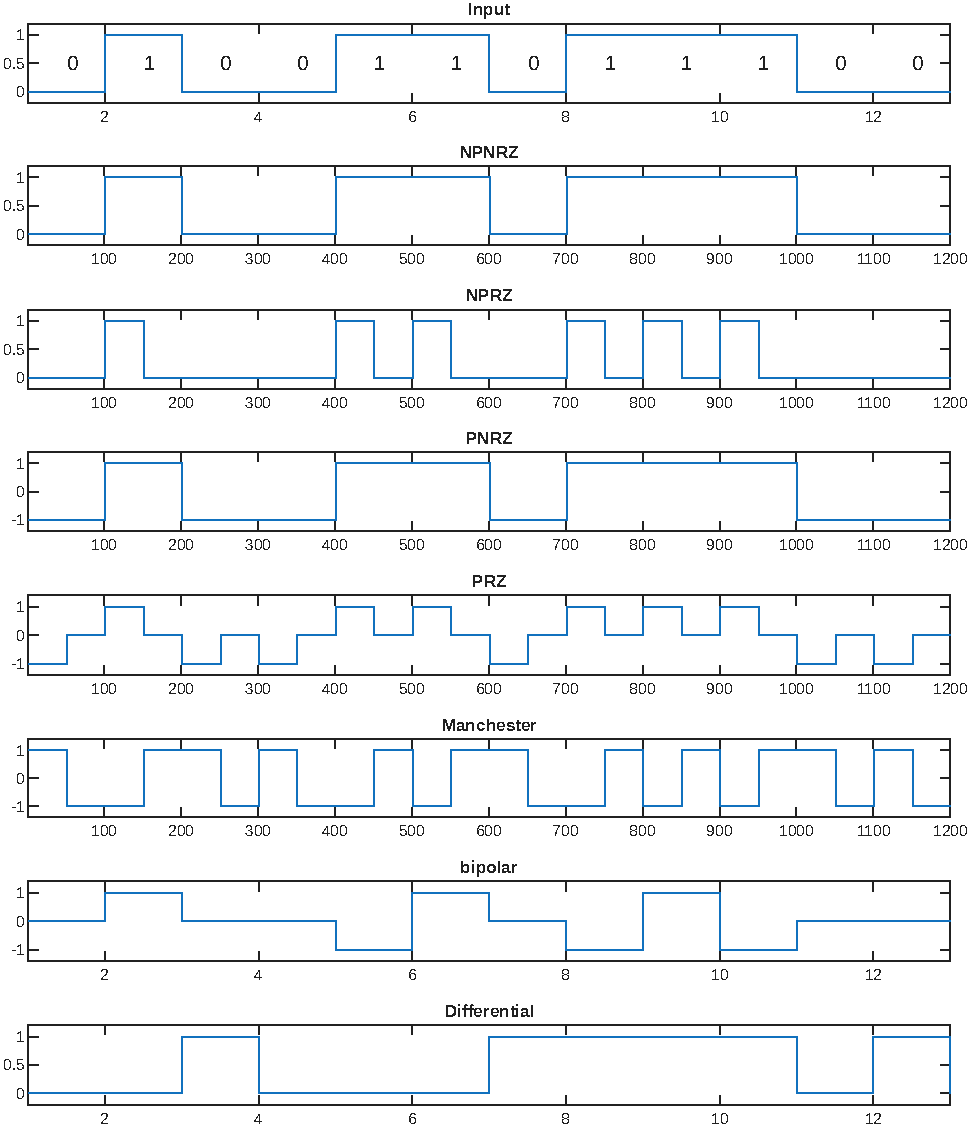
\includegraphics[width=0.9\linewidth]{img/linecode.pdf}
\end{figure}